\documentclass[10pt,a4paper]{article}
\usepackage[utf8]{inputenc}
\usepackage{amsmath}
\usepackage{float}
\usepackage{amsfonts}
\usepackage{amssymb}
\usepackage{graphicx}
\usepackage{cite}
\usepackage{hyperref}

\graphicspath{ {./images/} }

\title{US Spine Simulation and Results}

\author{Rui Xu \\ MBP rotation\\ Sept 8-Oct 14}

\begin{document}
\maketitle
 \newpage

\section*{Introduction}

This document will informally outline my ultrasound code and results. I have constructed a simple two-dimensional simulation using existing code from the k-wave package. The eventual goal is to simulate ultrasound propagation through vertebrae and optimize a set of transducers to deliver ultrasound to the spinal cord. 

\section*{The k-wave Toolbox}

I'll start with an overview of the k-wave code for my own understanding and benefit. Feel free to skip this section. 

\subsection*{Governing equations for acoustic (compressional) propagation}

The k-wave toolbox is used to simulate the propagation of pressure waves through media, which is described by a set of couple first-order partial differential equations or the wave equation, a second-order partial differential equation. K-wave uses the first order equation, 
\begin{align}
\dfrac{\partial \textbf{u}}{\partial t} &= - \frac{1}{\rho_0} \nabla p\\
\dfrac{\partial p }{\partial t} &= - \rho_0 \nabla \cdot \textbf{u}\\
p &= c_0^2 \rho
\end{align}
where \textbf{u} is particle velocity, $p$ is acoustic pressure, $\rho$ is acoustic density, $\rho_0$ is equilibrium acoustic density, and $c_0$ is the isentropic speed of sound. In words, the change in particle velocity is given by the pressure gradient, divided by equilibrium acoustic density. That is, particle velocity will increase in the direction down the pressure gradient, and this increase is inversely proportional to the equilibrium acoustic density. This is the equation of momentum conservation. The second equation states that the change in acoustic density is proportional to equilibrium particle density times the divergence of the particle velocity field (particle flux). This is the equation of mass conservation. Finally, we have the pressure - density relationship, where pressure is equal to the isentropic speed of sound ($c_0 = \sqrt{K_s/\rho_0}$, $K_s$ is the isentropic bulk modulus, squared, times the density at that location. 

This set of equations in this forms assumes that the medium is isotropic and quiescent. However, these equations must include additional terms if the medium is anisotropic and has absorbent properties, as shown in the following equations:
\begin{align}
\dfrac{\partial \textbf{u}}{\partial t} &= - \frac{1}{\rho_0} \nabla p\\
\dfrac{\partial p }{\partial t} &= - \rho_0 \nabla \cdot \textbf{u} - \textbf{u}\cdot \nabla \rho_0 \\
p &= c_0^2 (\rho + \textbf{d}\cdot\nabla \rho_0 -\textbf{L}\rho)
\end{align}
In this case, the momentum conservation equation remains the same. An additional term is present in the mass conservation equation to represent the additional mass transfer due to inhomogeneity in the equilibrium density profile of the medium (resulting in a non-zero gradient in $\rho_0$). The pressure-density relationship changes significantly, with the addition of the inner product of acoustic particle displacement \textbf{d} with the gradient of $\rho_0$, as well as a linear integro-differential operator ` \textbf{L}' that accounts for acoustic absorption $\alpha$) and dispersion in a medium that follows a frequency power law ($\alpha = \alpha_0 \omega^y$)  . This operator is defined:
\begin{equation}\label{Powerlawabsorption}
\textbf{L} = \tau \frac{\partial}{\partial t} ( - \nabla^2)^{\frac{y}{2} - 1} + \eta (-\nabla^2)^{\frac{y+1}{2} -1}
\end{equation}
where $\tau$ and $\eta$ are the absorption and dispersion proportionality coefficients:
\begin{equation}
\tau = -2\alpha_0c_0^{y-1}, \quad \quad \quad \eta = 2 \alpha_0c_0^y \tan \left(\frac{\pi y}{2} \right)
\end{equation}
where $\alpha_0$ is the power law pre-factor and $y$ is the power law exponent. 

Acoustic wave propagation ceases to be linear in certain biological circumstances, and in this case the governing equations of the system must be modified with higher order terms. k-Wave includes two non-linear terms   encompassed by a nonlinearity parameter $B/A$, which characterizes the contribution of finite-amplitude effects to sound speed. The governing equations are now:
\begin{align}
\dfrac{\partial \textbf{u}}{\partial t} &= - \frac{1}{\rho_0} \nabla p\\
\dfrac{\partial p }{\partial t} &= - (2<rho+\rho_0) \nabla \cdot \textbf{u} - \textbf{u}\cdot \nabla \rho_0 \\
p &= c_0^2 \left(\rho + \textbf{d}\cdot\nabla \rho_0 + \dfrac{B}{2A} \dfrac{\rho^2}{\rho_0}-\textbf{L}\rho\right)
\end{align}

We can generate acoustic waves in a medium by adding a force source term \textbf{S$_\textbf{F}$} to the momentum conservation equation and a mass source term and a mass source term \textbf{S$_\textbf{M}$} to the mass conservation equation.

\subsection*{Governing equations for shear wave propagation}

The k-wave toolbox is also able to simulate the propagation of elastic waves, which will be useful for understanding ultrasound propagation through bone. The k-wave code for compressional and shear wave propagation through elastic media is based on the Kelvin-Voight Model, which for an isotropic model is:
\begin{equation} \label{Kelvinvoight}
\sigma_{ij} = \lambda \delta_{ij} \epsilon_{kk} + 2 \mu \epsilon_{ij} + \chi \delta_{ij} \dfrac{\partial}{\partial t} \epsilon_{kk} + 2 \eta \dfrac{\partial}{\partial t} \epsilon_{ij} 
\end{equation}
where $\sigma$ is the stress tensor, $\epsilon$ is the strain tensor, $\lambda$ and $\mu$ are the Lam\'{e} parameters where $\mu$ is the shear modulus and $\chi$ and $\eta$ are the compressional and shear viscosity coefficients. The relationship between shear modulus and density is $\mu = c_s^2\rho_0$ and the relationship between Lam\'{e}'s first parameter, shear modulus, and density is $\lambda = c_p^2 \rho_0 - 2 \mu$. In these relationships, $c_s$ is the shear speed of sound and $c_p$ is the compressional speed of sound. \autoref{Kelvinvoight} states that the relationship between stress and instantaneous strain is parametrized by the Lam\'{e} parameters and the time dependency of the relationship is given by temporal derivatives of strain, which are parametrized by the compressional and shear viscosity coefficients. \autoref{Kelvinvoight} can be rewritten using the relationship between strain and small particle displacements $u_i$:
\begin{equation}
\epsilon_{ij} = \dfrac{1}{2} \left(\dfrac{\partial u_i}{\partial x_j} + \dfrac{\partial u_j}{\partial x_i} \right)
\end{equation}
which allows \autoref{Kelvinvoight} to be rewritten as a function of particle velocity $v_i = \partial u_i / \partial t$:
\begin{equation} \label{Kelvinvoightvelocity}
\dfrac{\partial \sigma_{ij}}{\partial t} = \lambda \delta_{ij} \dfrac{\partial v_k}{\partial x_k} + \mu \left( \dfrac{\partial v_i}{\partial x_j} + \dfrac{\partial v_j}{\partial x_i} \right) + \chi \delta_{ij} \dfrac{\partial^2 v_k}{\partial x_k \partial t} + \eta \left(\dfrac{\partial^2 v_i}{\partial x_j \partial t} + \dfrac{\partial^2 v_j}{\partial x_i \partial t} \right) 
\end{equation}
\autoref{Kelvinvoightvelocity} and an equation for the conservation of momentum:
\begin{equation}
\dfrac{\partial v_i}{\partial t} = \dfrac{1}{\rho_0} \dfrac{\partial \sigma_{ij}}{\partial x_j}
\end{equation}
are the coupled first order partial differential equations that we use to model the propagation of linear compressional and shear waves in an isotropic viscoelastic solid. The power law pre-factors for compressional and shear absorption ($\alpha_{0,p}$ and $\alpha_{0,s}$) in elastic media without high loss are given by:
\begin{equation}
\alpha_{0,p} = \dfrac{\chi + 2 \eta}{2 \rho_0 c_p^3}, \quad \quad \quad \alpha_{0,s} = \dfrac{\eta}{2\rho_0 c_s^3}
\end{equation}
This set of governing equations for ultrasound propagation in elastic media are solved in the same manner as in fluid media - by using a Pseudospectral Time Domain method. 

\subsection*{Pseudospectral method}

The k-wave toolbox uses a $k$-space pseudospectral method for the calculation of spatial derivatives, and then uses a finite difference scheme for temporal updates. For example, we can take the wave equation system for a simple homogeneous and lossless system,
\begin{equation}
\nabla^2 p (\textbf{x},t) - \dfrac{1}{c_0^2} \dfrac{\partial^2}{\partial t^2} p (\textbf{x},t)
\end{equation}
and use a spatial Fourier transform to rewrite the equation in $k$-space where it has the form:
\begin{equation}
\frac{\partial^2}{\partial t^2} p(\textbf{k},t) = - (c_0 k)^2 p(\textbf{k},t)
\end{equation}
and we can rewrite the temporal derivative as:
\begin{equation}
\frac{\partial^2}{\partial t^2} p(\textbf{k},t) = \dfrac{p(\textbf{k},t+\Delta t) - 2p(\textbf{k},t)+p(\textbf{k}, t-\Delta t)}{\Delta t^2} = - (c_0 k)^2 p(\textbf{k},t)
\end{equation}
This finite difference approximation scheme is subject to dispersion for large scale simulations, and this dispersion results in the accumulation of phase errors. However, we can replace the $\Delta t^2$ term by multiplying a corrective operator, the $k$-space operator, $\kappa^2 = \text{sinc}^2(c_{\text{ref}} k \Delta t/2)$. This technique is described in the textbook `Nonstandard Finite Difference Models of Differential Equations', \cite{mickens1993nonstandard}. Another approach k-wave uses to increase the stability and accuracy of the simulation is by using staggered spatial and temporal grids. 

\subsection*{Discretized equations}

The mass and momentum equations, written in discrete form and using the k-space pseudospectral method, have the following form:
\begin{align}
\dfrac{\partial}{\partial \xi} p^n &= \mathcal{F}^{-1} \left[ i k_{\xi} \kappa e^{ i k_{\xi} \Delta \xi /2} \mathcal{F} \left[ p^n \right] \right] \\
u_{\xi}^{n+\frac{1}{2}} &= u_{\xi}^{n-\frac{1}{2}} - \dfrac{\Delta t}{\rho_0} \dfrac{\partial}{\partial \xi} p^n + \Delta t \textbf{S}_{\textbf{F}_{\xi}}^n\\
\dfrac{\partial}{\partial \xi} u_{\xi}^{n+\frac{1}{2}} &= \mathcal{F}^{-1} \left[ i k_{\xi} \kappa e^{-ik_{\xi} \Delta \xi / 2} \mathcal{F} \left[ u_{\xi}^{n+\frac{1}{2}} \right] \right]\\
\rho_{\xi}^{n+1} &= \rho_{\xi}^n - \Delta t \rho_0 \dfrac{\partial}{\partial \xi} u_{\xi}^{n+\frac{1}{2}} + \Delta t  \textbf{S}_{\textbf{F}_{\xi}}^{n+\frac{1}{2}}
\end{align}
In the above, the first and third equations are spatial gradient calculations and the second and fourth equations are update steps. The symbol $\xi$ represents Cartesian coordinates for one to three dimensional systems, $k_{\xi}$ represents wavenumber in the $\xi$ direction and is discretized according to: 
\begin{equation}
k_{\xi} = \left[-\dfrac{\text{N}_{\xi}}{2}, -\dfrac{\text{N}_{\xi}}{2}+1, ... , \dfrac{\text{N}_{\xi}}{2} -1 \right] \dfrac{2\pi}{\Delta \xi \textbf{N}_{\xi}}
\end{equation}
if N$_{\xi}$ is even, or 
\begin{equation}
k_{\xi} = \left[-\dfrac{\text{N-1}_{\xi}}{2}, -\dfrac{\text{N-1}_{\xi}}{2}+1, ... , \dfrac{\text{N-1}_{\xi}}{2} \right] \dfrac{2\pi}{\Delta \xi \textbf{N}_{\xi}}
\end{equation}
if N$_{\xi}$ is odd. The algorithm follows a simple procedure, where pressure is known at timestep $n$, then pressure differentials are calculated at staggered grid points for this timestep $n$. Subsequently, particle velocity is calculated from these pressure differentials for timestep $n+1/2$ at the staggered grid points. Next, velocity differentials area calculated at the regular grid points, and these velocity differentials are subsequently used to update density (and therefore pressure using the pressure-density relation) at the regular grid points for timestep $n+1/2$. The discretized pressure-density relation is $p^{n+1} = c_0^2(\rho^{n+1} - \textbf{L}_{\text{d}}$, where L$_{\text{d}}$ is the discretized form of the power law absorption term (Equation \ref{Powerlawabsorption}). The discretized form of the power law absorption term is:
\begin{align}
\text{L}_{\text{d}} &= \tau \mathcal{F}^{-1} \left[k^{y-2} \mathcal{F} \left[\frac{\partial}{\partial t} \rho^n \right] \right] + \eta \mathcal{F}^{-1} \left[ k^{y-1} \mathcal{F}\left[\rho^{n+1}\right] \right]\\
&= \tau \mathcal{F}^{-1} \left[k^{y-2} \mathcal{F} \left[\rho_0 \sum_{\xi} \frac{\partial}{\partial \xi} x_{\xi}^{n+\frac{1}{2}} \right] \right] + \eta \mathcal{F}^{-1} \left[ k^{y-1} \mathcal{F}\left[\rho^{n+1}\right] \right]
\end{align}

The method is similar for the elastic simulation. The spatial gradients of the stress field are first calculated using the Fourier collocation spectral method. Next, the particle velocities are updated using a finite difference time step. Then, the spatial gradients of the velocity field is calculated using the Fourier collocation spectral method, and then the spatial gradient of the time derivative of the particle velocity is calculated. Finally, the stress field is updated using the results from the previous steps. 

\subsection*{Accuracy of the simulation}

The accuracy of the model depends on the spatial and temporal discretization ($\Delta x, \Delta y$). Given that the model is correct and the simulation stability ensured by choosing a reasonable Courant-Friedrichs-Lewy number (CFL $\equiv c_0 \Delta t /\Delta x$ (e.g. 0.3 for weakly heterogeneous media), then the model should converge to the solution to the continuous equations in the limit where $\Delta x$ and $\Delta t$ go to zero. However, it is not possible to do this in practice due to finite computing resources. Instead, we choose $\Delta x$ such that the maximum frequencies of interest are supported on the grid, and $\Delta t$ short enough that decreasing it will not cause any change in the simulation results. Decreasing $\Delta t$ improves the accuracy for propagation across an interface, and therefore will important to consider for this work. 

Smoothing of a discretized system - sharp discontinuities in the spatial domain have a broad spectrum in the spatial frequency domain. The go-to example for this relationship is the spatial delta function, for which the frequency response is 1. This means that high energy, high frequency components are highly represented in the solution, which results in oscillations in the solution that are commonly called `ringing'. It is possible to reduce ringing in the solution by applying smoothing functions such as the Hanning window or Blackman window. 
\section*{System 1: Homogeneous Medium, Two Elements, Two Frequencies}

The first system I created was a system of two curved transducers, each with a radius of curvature of 50mm, and each subtending $\pi/2$ radians. The two transducers are driven at frequencies $f_1$ and $f_2$. The focal point of the two transducers are the same. I create the transducers by defining source points at a 50mm radius for $\pi/12 \leq \Theta_1 \leq 5\pi/12$ and $7\pi/12 \leq \Theta_2 \leq 11 \pi/12$. The system setup is shown in \autoref{setup1}.

\begin{figure}[!h]
\centering
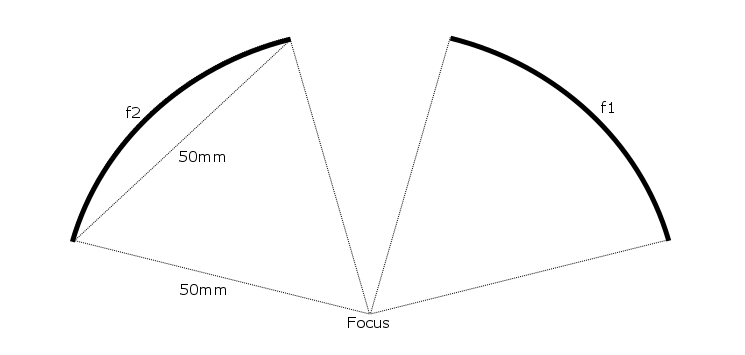
\includegraphics[scale=0.5]{setup1.png}
\caption{This system has two curved transducers with 50mm focal lengths, located such that the focal points of the two transducers are the same.} \label{setup1}
\centering
\end{figure}

\subsection*{Half-Maximum Profiles}

The first test was to vary the frequency $f_1$ of the right hand side transducer, while keeping the frequency of the second transducer constant $f_2 = 0.25$MHz. Implementing multiple frequencies in k-wave require that each source point have its frequency assigned to it. In the current implementation, I've looped over all points, and set the frequency of the source points on the left half of the computational box to $f_2$ and those on the right half to $f_1$. Take care with the current code if you move the transducers around. It might be a good idea to write a foolproof version of the frequency assignment part of the code, perhaps by combining it with the code that builds the source mask.\\

We are interested in the pressure profile of the system near the focal point, for different frequencies $0.15 \text{MHz} \leq f_1 \leq 0.35 \text{MHz}$, tested in increments of 10kHz. The following figures show the 2D root-mean-square pressure profiles. The points of half-maximum pressure are outlined in black.

\begin{figure}[!h]\label{f150kHz}
\hspace*{-5cm}                                                    
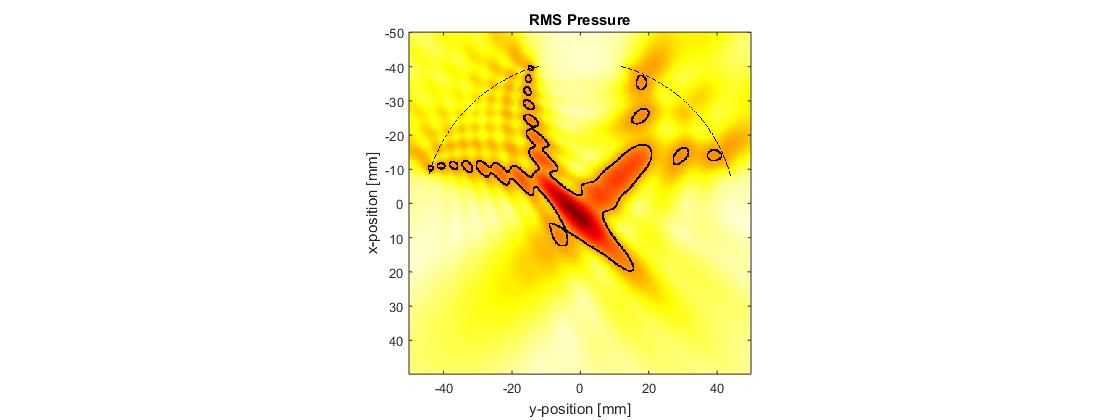
\includegraphics[scale=0.6]{f150kHz}
\caption{RMS pressure profile for $f_1 = 0.15$MHz, $f_2 = 0.25$MHz}
\end{figure}
\begin{figure}[!h]\label{f160kHz}
\hspace*{-5cm}                                                    
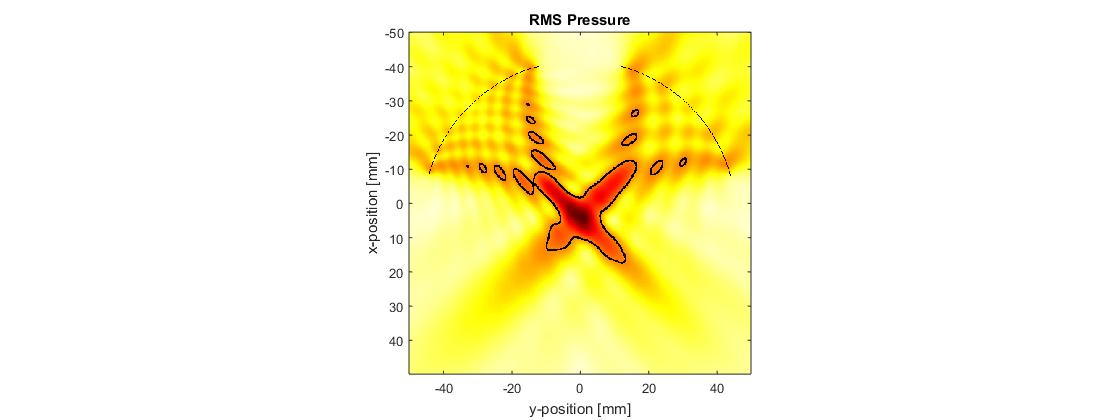
\includegraphics[scale=0.6]{f160kHz}
\caption{RMS pressure profile for $f_1 = 0.16$MHz, $f_2 = 0.25$MHz}
\end{figure}
\begin{figure}[!h]\label{f170kHz}
\hspace*{-5cm}                                                    
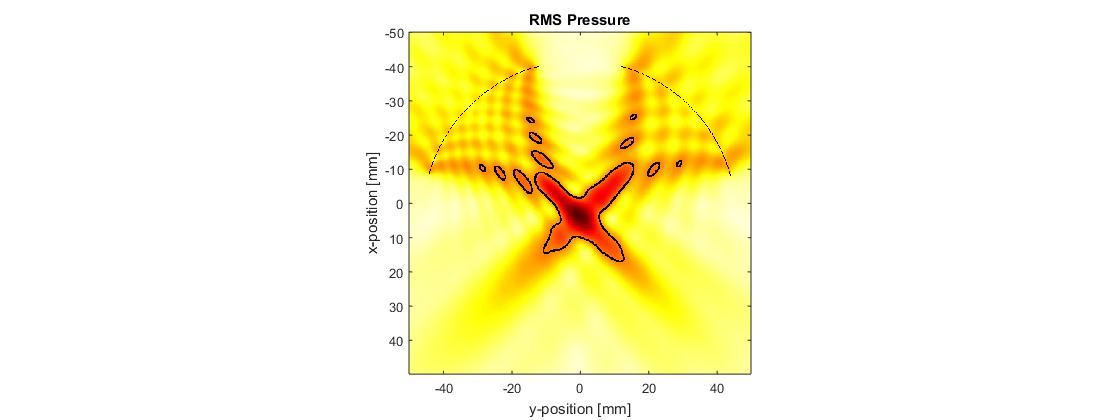
\includegraphics[scale=0.6]{f170kHz}
\caption{RMS pressure profile for $f_1 = 0.17$MHz, $f_2 = 0.25$MHz}
\end{figure}
\begin{figure}[!h]\label{f180kHz}
\hspace*{-5cm}                                                    
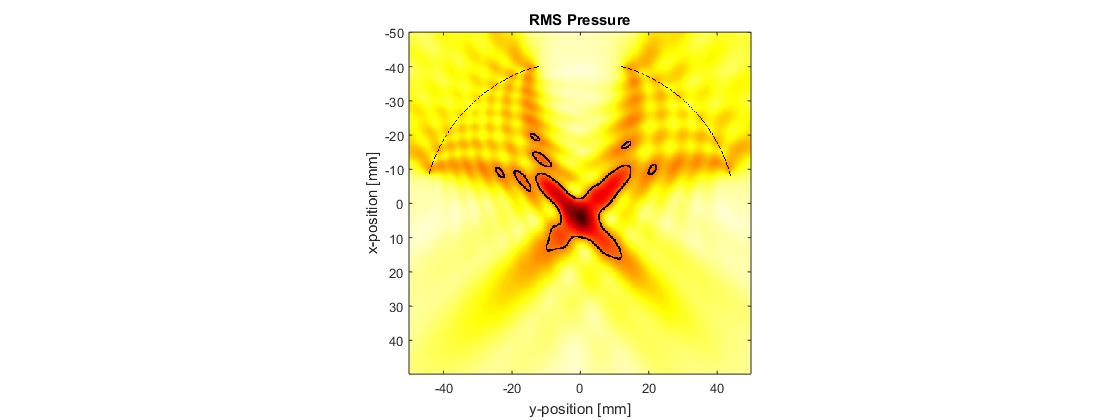
\includegraphics[scale=0.6]{f180kHz}
\caption{RMS pressure profile for $f_1 = 0.18$MHz, $f_2 = 0.25$MHz}
\end{figure}
\begin{figure}[!h]\label{f190kHz}
\hspace*{-5cm}                                                    
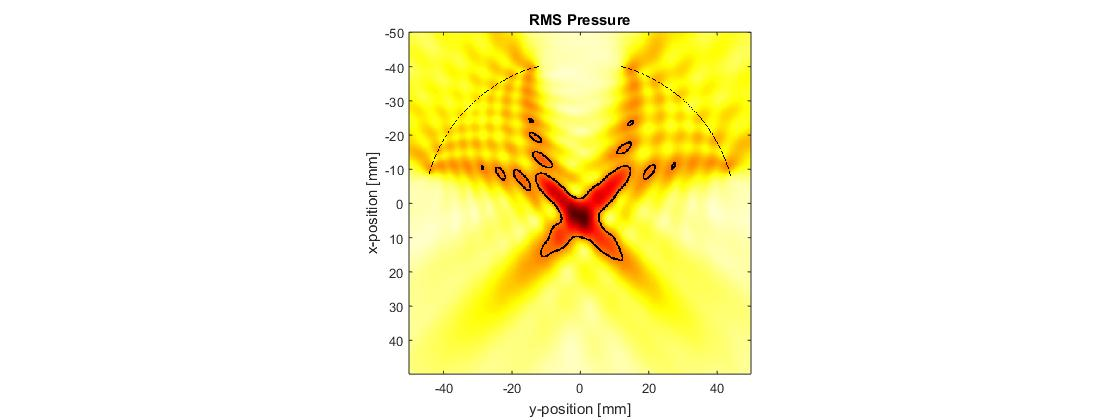
\includegraphics[scale=0.6]{f190kHz}
\caption{RMS pressure profile for $f_1 = 0.19$MHz, $f_2 = 0.25$MHz}
\end{figure}
\begin{figure}[!h]\label{f200kHz}
\hspace*{-5cm}                                                    
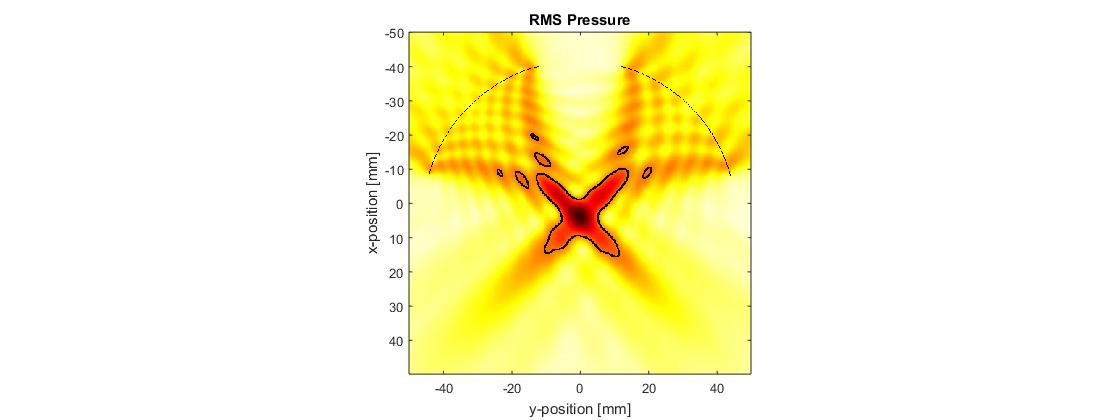
\includegraphics[scale=0.6]{f200kHz}
\caption{RMS pressure profile for $f_1 = 0.20$MHz, $f_2 = 0.25$MHz}
\end{figure}
\begin{figure}[!h]\label{f210kHz}
\hspace*{-5cm}                                                    
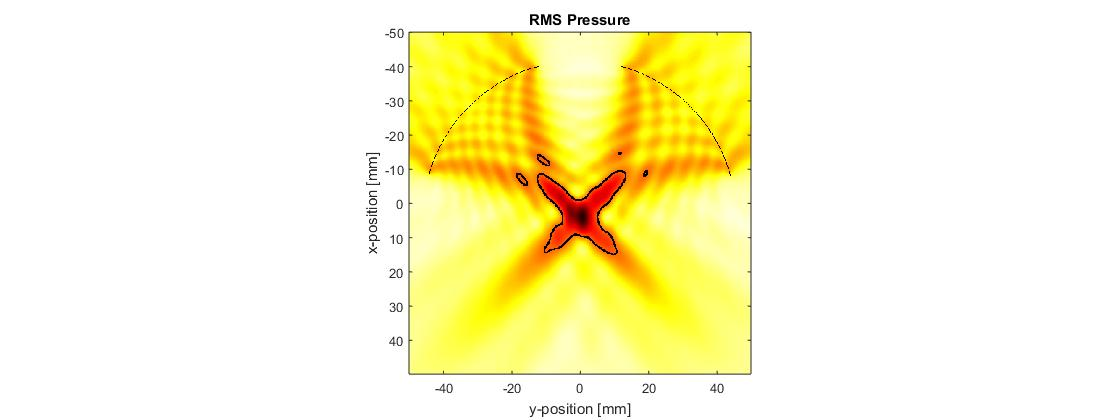
\includegraphics[scale=0.6]{f210kHz}
\caption{RMS pressure profile for $f_1 = 0.21$MHz, $f_2 = 0.25$MHz}
\end{figure}
\begin{figure}[!h]\label{f220kHz}
\hspace*{-5cm}                                                    
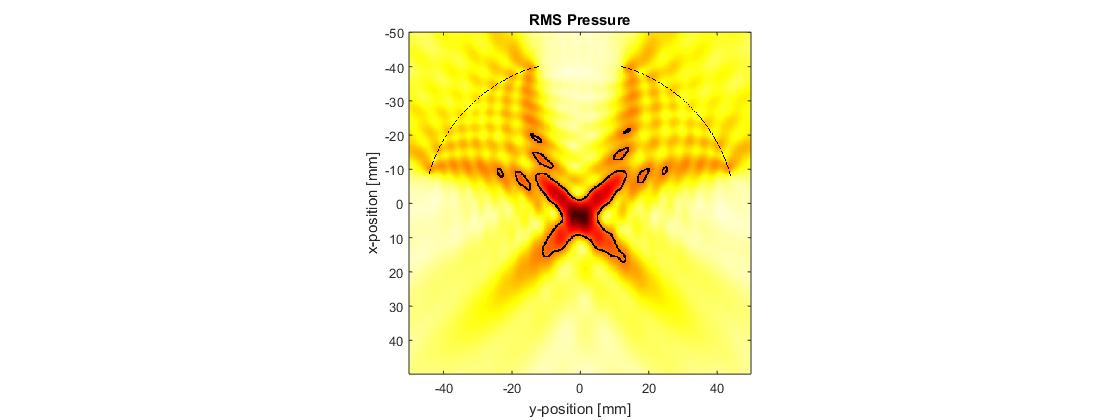
\includegraphics[scale=0.6]{f220kHz}
\caption{RMS pressure profile for $f_1 = 0.22$MHz, $f_2 = 0.25$MHz}
\end{figure}
\begin{figure}[!h]\label{f230kHz}
\hspace*{-5cm}                                                    
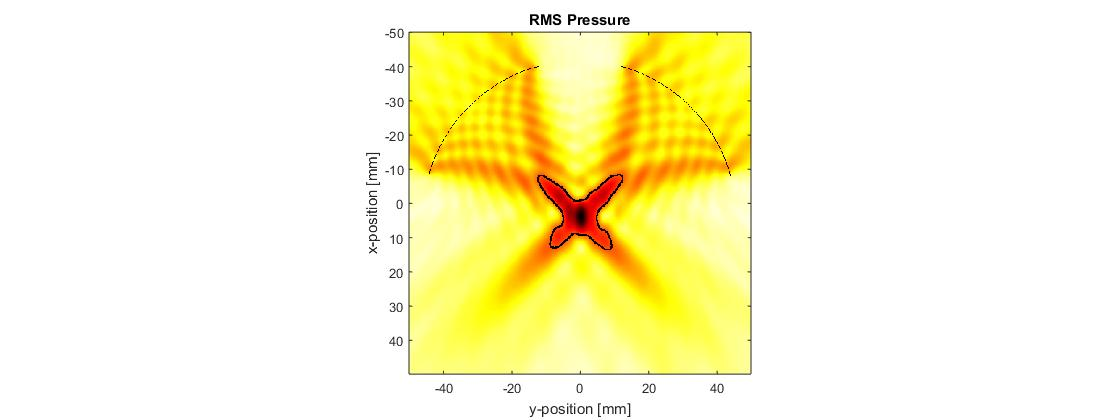
\includegraphics[scale=0.6]{f230kHz}
\caption{RMS pressure profile for $f_1 = 0.23$MHz, $f_2 = 0.25$MHz}
\end{figure}
\begin{figure}[!h]\label{f240kHz}
\hspace*{-5cm}                                                    
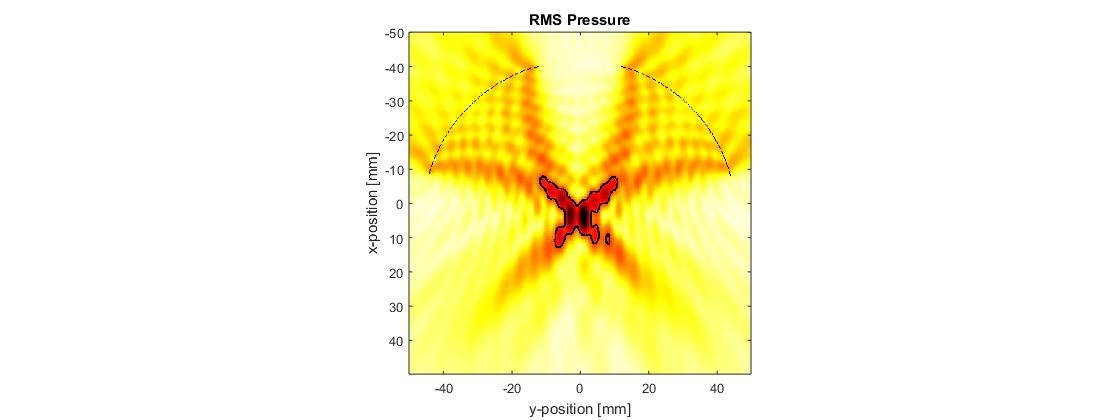
\includegraphics[scale=0.6]{f240kHz}
\caption{RMS pressure profile for $f_1 = 0.24$MHz, $f_2 = 0.25$MHz}
\end{figure}
\begin{figure}[!h]\label{f250kHz}
\hspace*{-5cm}                                                    
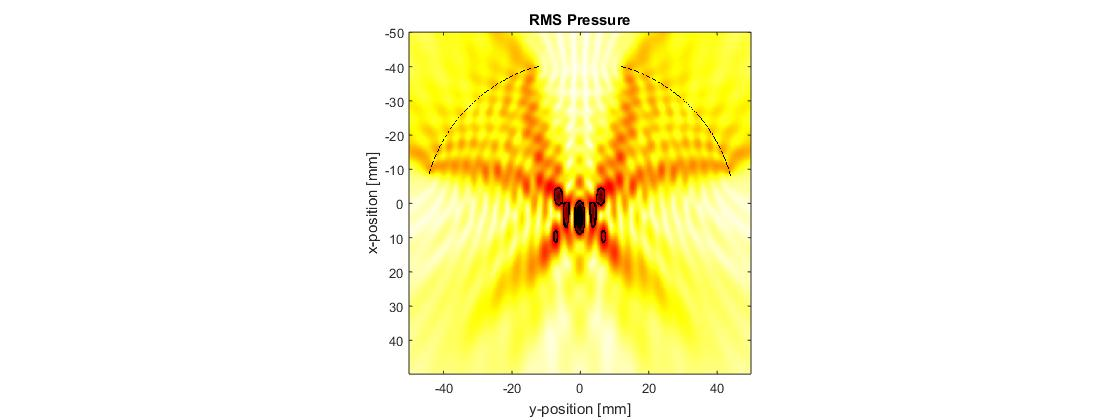
\includegraphics[scale=0.6]{f250kHz}
\caption{RMS pressure profile for $f_1 = 0.25$MHz, $f_2 = 0.25$MHz}
\end{figure}
\begin{figure}[!h]\label{f260kHz}
\hspace*{-5cm}                                                    
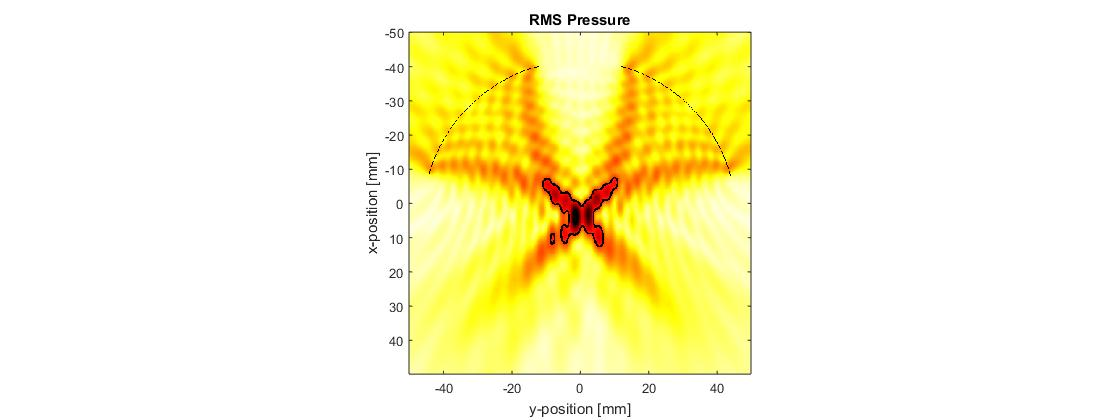
\includegraphics[scale=0.6]{f260kHz}
\caption{RMS pressure profile for $f_1 = 0.26$MHz, $f_2 = 0.25$MHz}
\end{figure}
\begin{figure}[!h]\label{f270kHz}
\hspace*{-5cm}                                                    
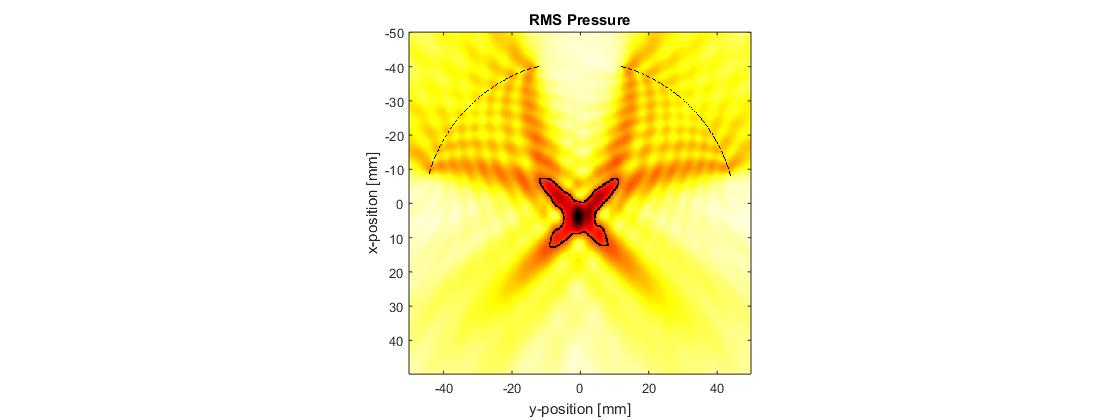
\includegraphics[scale=0.6]{f270kHz}
\caption{RMS pressure profile for $f_1 = 0.27$MHz, $f_2 = 0.25$MHz}
\end{figure}
\begin{figure}[!h]\label{f280kHz}
\hspace*{-5cm}                                                    
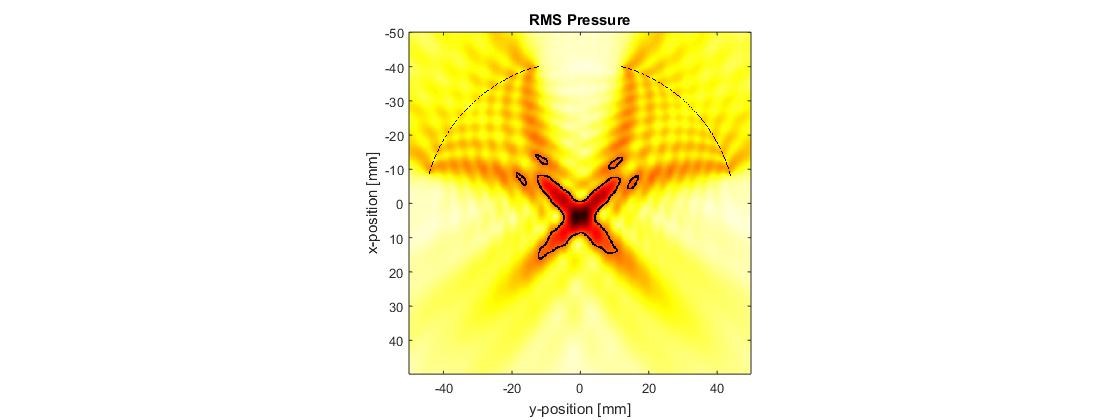
\includegraphics[scale=0.6]{f280kHz}
\caption{RMS pressure profile for $f_1 = 0.28$MHz, $f_2 = 0.25$MHz}
\end{figure}
\begin{figure}[!h]\label{f290kHz}
\hspace*{-5cm}                                                    
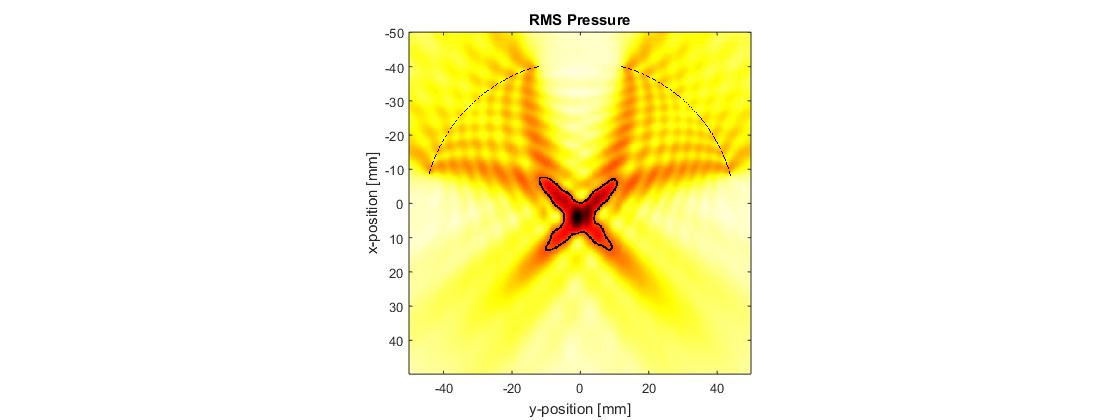
\includegraphics[scale=0.6]{f290kHz}
\caption{RMS pressure profile for $f_1 = 0.29$MHz, $f_2 = 0.25$MHz}
\end{figure}
\begin{figure}[!h]\label{f300kHz}
\hspace*{-5cm}                                                    
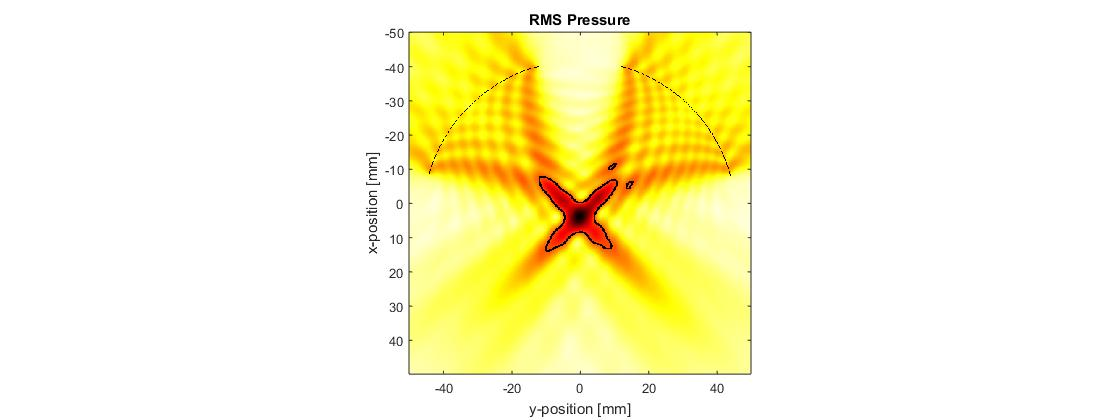
\includegraphics[scale=0.6]{f300kHz}
\caption{RMS pressure profile for $f_1 = 0.30$MHz, $f_2 = 0.25$MHz}
\end{figure}
\begin{figure}[!h]\label{f310kHz}
\hspace*{-5cm}                                                    
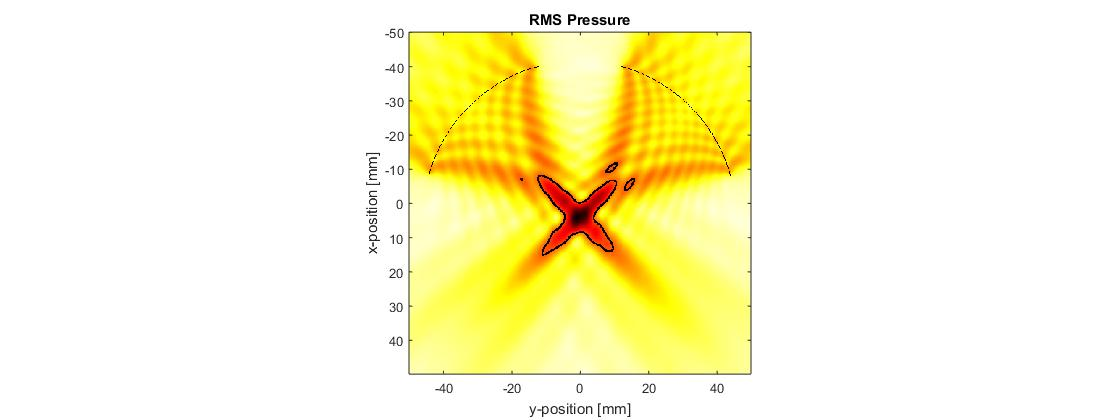
\includegraphics[scale=0.6]{f310kHz}
\caption{RMS pressure profile for $f_1 = 0.31$MHz, $f_2 = 0.25$MHz}
\end{figure}
\begin{figure}[!h]\label{f320kHz}
\hspace*{-5cm}                                                    
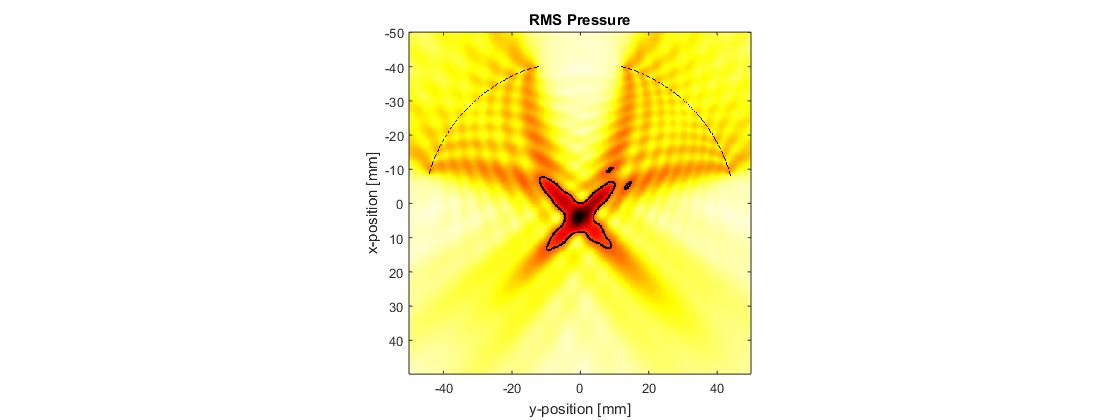
\includegraphics[scale=0.6]{f320kHz}
\caption{RMS pressure profile for $f_1 = 0.32$MHz, $f_2 = 0.25$MHz}
\end{figure}
\begin{figure}[!h]\label{f330kHz}
\hspace*{-5cm}                                                    
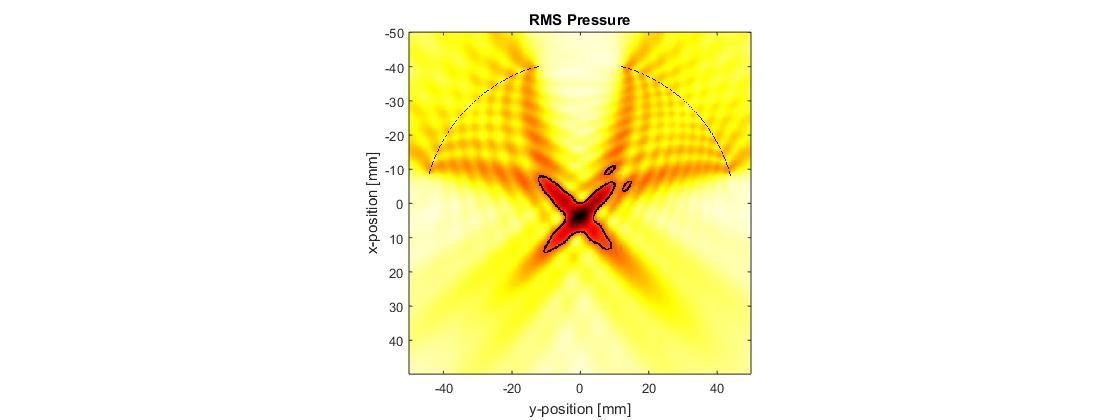
\includegraphics[scale=0.6]{f330kHz}
\caption{RMS pressure profile for $f_1 = 0.33$MHz, $f_2 = 0.25$MHz}
\end{figure}
\begin{figure}[!h]\label{f340kHz}
\hspace*{-5cm}                                                    
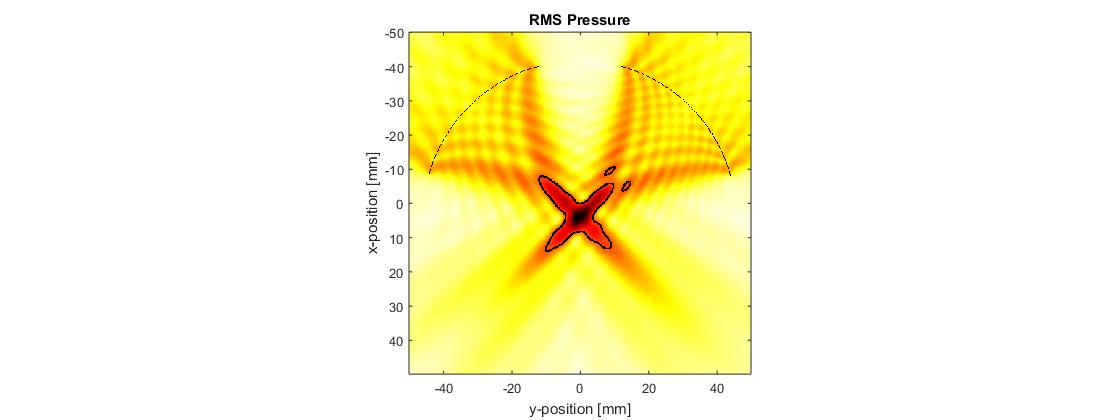
\includegraphics[scale=0.6]{f340kHz}
\caption{RMS pressure profile for $f_1 = 0.34$MHz, $f_2 = 0.25$MHz}
\end{figure}
\begin{figure}[!h]\label{f350kHz}
\hspace*{-5cm}                                                    
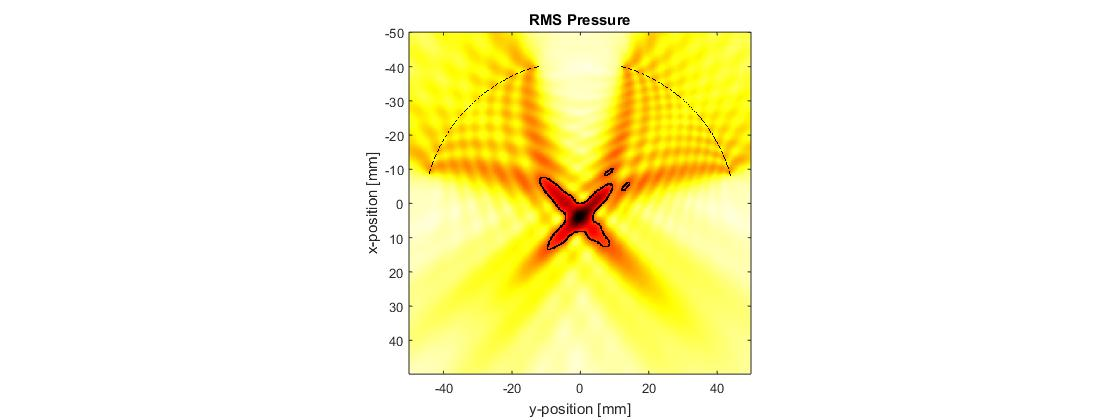
\includegraphics[scale=0.6]{f350kHz}
\caption{RMS pressure profile for $f_1 = 0.35$MHz, $f_2 = 0.25$MHz}
\end{figure}
\newpage

\subsection*{FWHM for different frequencies}

An informative metric for (approximately) Gaussian pressure profiles is the Full Width at Half Maximum (FWHM). The method I used for finding the points with half maximum pressure returns coordinates for all points, not just those around the central maximum. This is remediable, but the profiles remain non-circulate. The FWHM of the distributions can easily be calculated from the coordinates ($x_{HM},y_{HM}$) by first calculating the coordinate of the centre of the HM points ($x_{HMc}, y_{HMc})$:
\begin{equation}
x_{HMc} = \frac{1}{N} \sum_{i=1}^N x_{HM_i} \cdot dx, \quad \quad x_{HMc} = \frac{1}{N} \sum_{i=1}^N x_{HM_i} \cdot dx
\end{equation}
where $N$ is the number of HM points. We can calculate the average distance $d$ of the HM points from the HM centre using:
\begin{equation}
d = \frac{1}{N}  \sum_{i=1}^N \sqrt{ (x_{HM_i} - x_{HMc})^2 + (y_{HM_i} - y_{HMc})^2} \cdot dx 
\end{equation}
The FWHM is then approximately equal to two times the average distance between an HM point and the centre of the HM point distribution. For HM distributions that are highly non-Gaussian, then there is little purpose in calling it the FWHM - it's simply the average width of the half-maximum RMS pressure profile. Despite this, I'll continue calling it FWHM for the time being. The FWHM is shown for 200kHz$\leq f_1 \leq$ 300kHz in Figure \ref{FWHM_freq}.

\begin{figure}[H]\label{FWHM_freq}
\centering
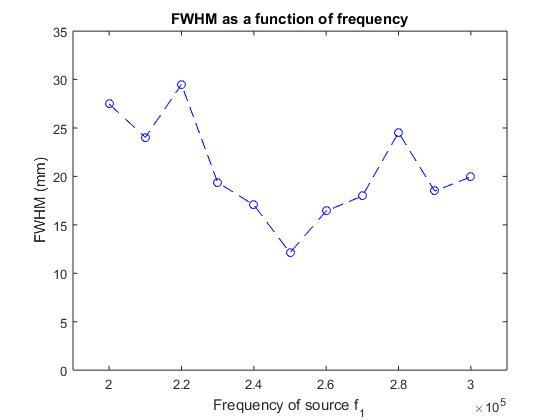
\includegraphics[scale=0.6]{FWHM_freq}
\caption{The FWHM of the RMS pressure distribution for 200kHz$\leq f_1 \leq$ 300kHz, $f_2 = 250$kHz.}
\end{figure}


\subsection*{Centre of HM profile}

I've included this for curiosity's sake. Here I plot the centre of the FWHM profile, for 200kHz$\leq f_1 \leq$ 300kHz.
\begin{figure}[H]\label{FWHM_centre}
\centering
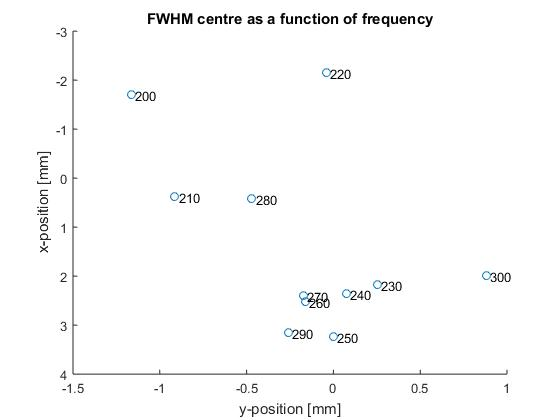
\includegraphics[scale=0.6]{FWHM_centre}
\caption{The coordinates of the centre of the FWHM profile of the RMS pressure distribution for 200kHz$\leq f_1 \leq$ 300kHz, $f_2 = 250$kHz. [0,0] is the coordinate of the focal point of the two transducers.}
\end{figure}

\subsection*{Maximum RMS Pressure}

We are also interested in the location of the maximum RMS intensity for different frequencies. These are shown in the following Figure \ref{RMS_Max}. 

\begin{figure}[H] \label{RMS_Max}
\centering
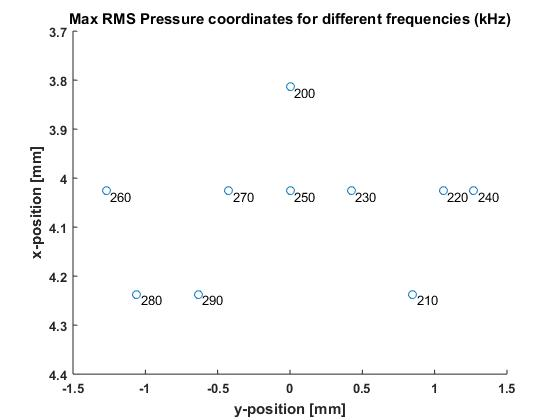
\includegraphics[scale=0.65]{Max_RMS_pressure_coords}
\caption{The Maximum RMS pressure location for 200kHz$\leq f_1 \leq$300kHz.  [0,0] is the coordinate of the focal point of the two transducers. } 
\end{figure}

There does not appear to be any pattern in the location of the maximum RMS pressure coordinates. In the x-dimension, the maxima are confined to within three computational grid points, approximately +4mm away from the focal point of the independent transducers. In the y-dimension, the maxima remain closely clustered around the focal point. Generally, the maximum RMS pressure is much more highly clustered than the FWHM centre.

\section*{System 2: Adding Inclusions}

The next step to increasing the complexity of the simulation is to add an inclusion near the focal point of the two transducers. The acoustic properties that k-wave includes are the sound speed within the medium, the ambient density distribution within the medium, a nonlinearity parameter, the power law absorption prefactor $\alpha_0$, and the power law absorption exponent $y$, where the power law is:
\begin{equation}
\alpha(f) = \alpha_0 \omega^y, 	\quad \omega = 2 \pi f 
\end{equation}

The simulation package, k-wave, doesn't include all non-linear effects, but does include two additional non-linear terms to attempt to account for all non-linear behaviour. These terms are defined as BonA in k-wave, where A and B are the first and second terms in the Taylor series expansion of the relation between the materials pressure and density.

All of these variables can be set as spatially heterogeneous in k-wave. In order to make an accurate simulation, I will need the acoustic properties of the medium I'll be simulating - namely water, bone, fat, nerve tissue, etc. Some of these are available in "Physical Properties of Tissue", a reference book by Francis A. Duck, and referenced by Chris Diederich in his interstitial spine simulation work \cite{duck1990physical}.

For this simulation, it will also be important to be able to account for shear wave propagation, as bone is a solid medium that supports shear wave propagation \cite{treeby2015contribution}. There is the option to use an updated file from k-wave called PSTDELASTIC2D that allows for the separation of the compressional and shear components of the ultrasound wave. The details of the algorithm used for the propagation of shear waves in elastic media are described in full in their paper `Modelling Elastic Wave Propagation Using the k-Wave MATLAB Toolbox' \cite{treeby2014modelling}.

In order to understand the effect of shear wave propagation in a bone, I built another simulation, starting from the k-wave Snell's law example. In this simulation I use a circular inclusion centred near the focal point of the two transducers such that the ultrasound waves intersect at the proximal side of the inclusion. I set the radius of the circular inclusion to 1cm, and set the compressional speed of sound to be $v_P = 2820$m/s, the shear speed of sound to $v_S$ = 1500m/s, the compressional alpha factor to $\alpha_P = 9$, and the shear alpha factor to $\alpha_S = 20$. In the rest of the simulation medium then I use $v_P = 1580$m/s, $v_s = 0$m/s, $\alpha_P = 0.57$, and $\alpha_S = 0$. I'm not sure if I should be setting $\alpha_S$ to zero, but since there should not be any shear waves propagating through the non-bone medium, then it should be a reasonable input. The set-up for this simulation is shown in \autoref{setup2}.
\begin{figure}[H] 
\centering
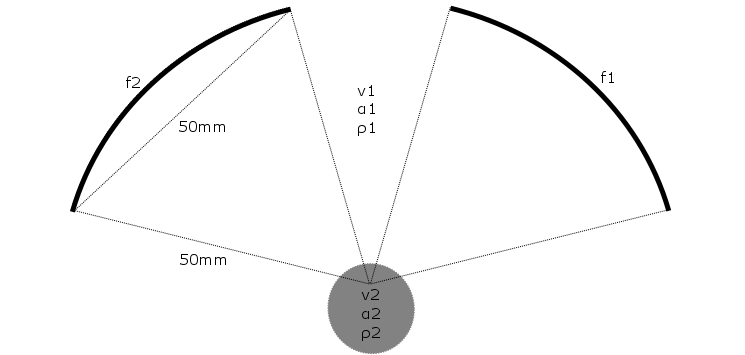
\includegraphics[scale=0.5]{setup2}
\caption{An inclusion is added to the system, with the same acoustic properties as those used by \cite{treeby2015contribution}.}\label{setup2}
\end{figure}

The code is set to run the fluid simulation first, and then run the elastic simulation after to allow for comparison between the two models. The results of the simulation are shown in Figure \ref{elasticvsfluid_heatmap}. In this figure, the quantity plotted is the logarithm of squared particle velocity, normalized by the maximum squared particle velocity $\vert \textbf{u} \cdot \textbf{u} \vert / \vert  \textbf{u}_{max} \cdot \textbf{u}_{max}\vert $. For this first test case, the frequencies of the two transducers are both 0.25MHz. 

\begin{figure}[H]
\centering
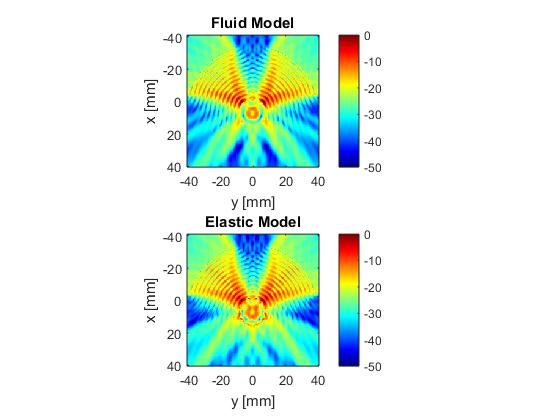
\includegraphics[scale=0.7]{circle_elasticvsfluid_heatmap}
\caption{In this figure, the logarithm of normalized, squared particle velocity is plotted for the fluid simulation and the elastic simulation. This quantity is proportional to heat deposition, where the proportionality constants are the speed of sound in the medium, the medium density, and the absorption coefficient of the medium. This quantity, thermal deposition, is important for thermal ultrasound applications.}\label{elasticvsfluid_heatmap}
\end{figure}

In \autoref{HM_elasticvsfluid} , the half-maximum contours of the RMS pressure profiles are outlined for both fluid and elastic simulations. It is somewhat difficult to see the HM lines in the figure because the pressure profiles are highly peaked. 

\begin{figure}[H]
\hspace*{-4cm}                                                    
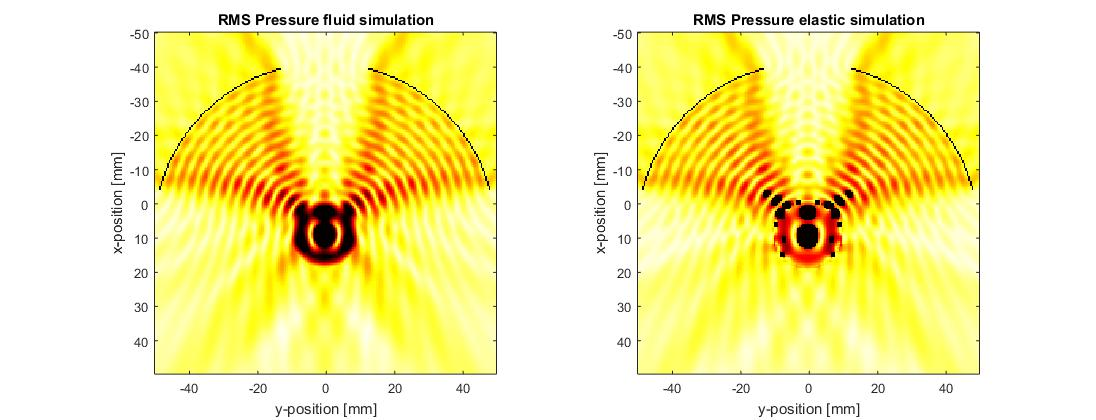
\includegraphics[scale=0.5]{FWHM_elasticvsfluid}
\label{HM_elasticvsfluid}
\end{figure}

\subsection*{Half-Maximum Profiles}

\begin{figure}[H]
\hspace*{-4cm}                                                    
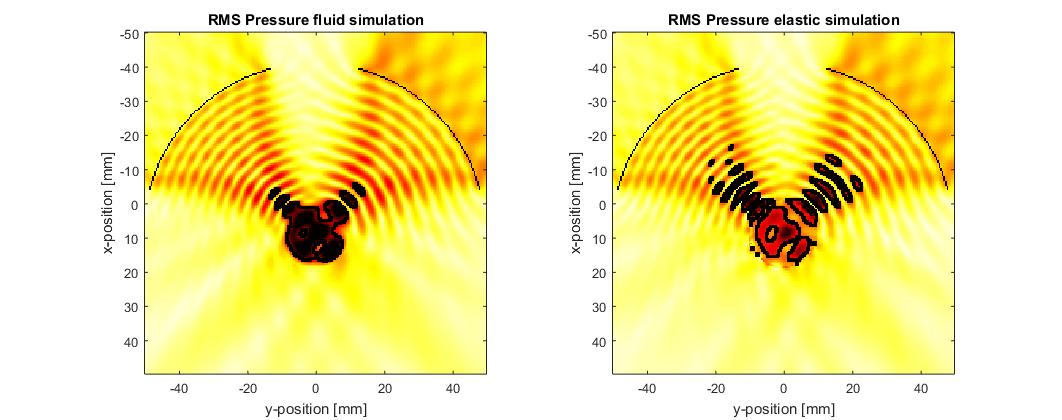
\includegraphics[scale=0.55]{comp_200kHz}
\caption{$f_1  = 0.2$Mhz, $f_2 = 0.25$Mhz.}
\label{comp_200kHz}
\end{figure}
\begin{figure}[H]
\hspace*{-4cm}                                                    
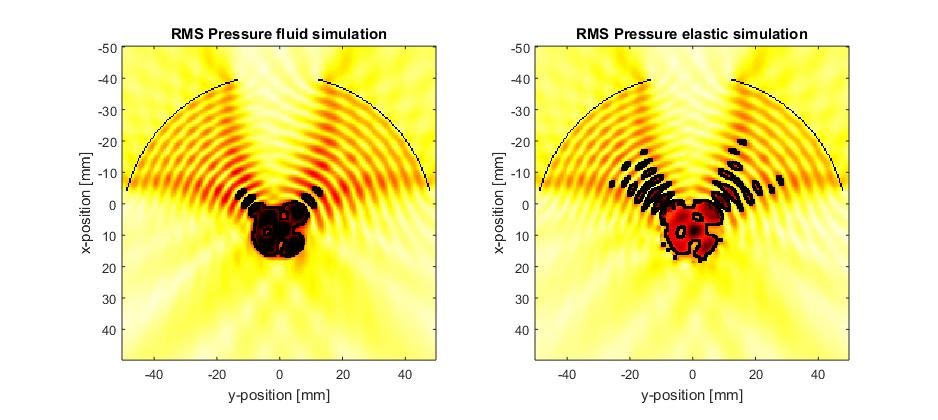
\includegraphics[scale=0.6]{comp_210kHz}
\caption{$f_1  = 0.21$Mhz, $f_2 = 0.25$Mhz.}
\label{comp_210kHz}
\end{figure}
\begin{figure}[H]
\hspace*{-4cm}                                                    
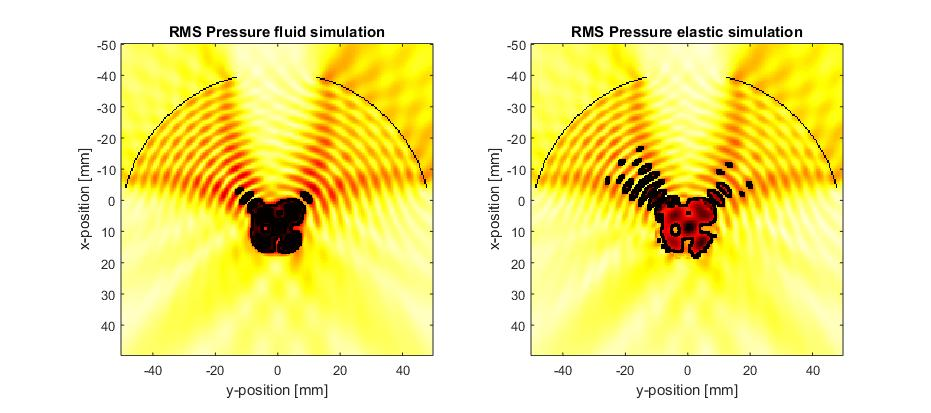
\includegraphics[scale=0.6]{comp_220kHz}
\caption{$f_1  = 0.22$Mhz, $f_2 = 0.25$Mhz.}
\label{comp_220kHz}
\end{figure}
\begin{figure}[H]
\hspace*{-4cm}                                                    
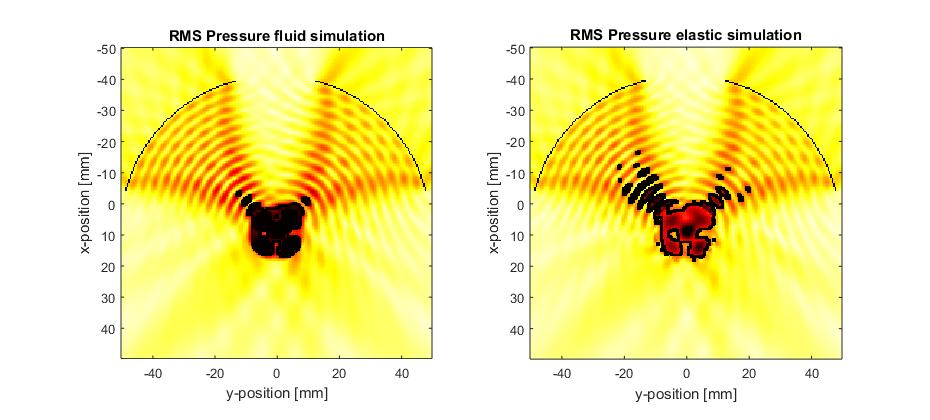
\includegraphics[scale=0.6]{comp_230kHz}
\caption{$f_1  = 0.23$Mhz, $f_2 = 0.25$Mhz.}
\label{comp_230kHz}
\end{figure}
\begin{figure}[H]
\hspace*{-4cm}                                                    
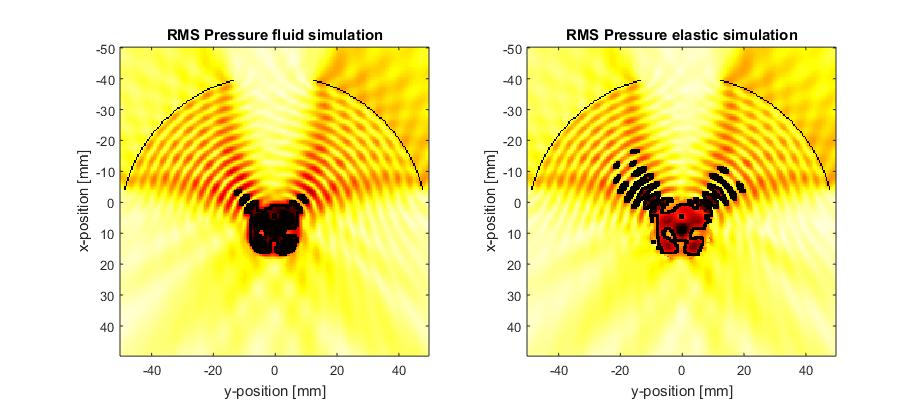
\includegraphics[scale=0.6]{comp_240kHz}
\caption{$f_1  = 0.24$Mhz, $f_2 = 0.25$Mhz.}
\label{comp_240kHz}
\end{figure}
\begin{figure}[H]
\hspace*{-4cm}                                                    
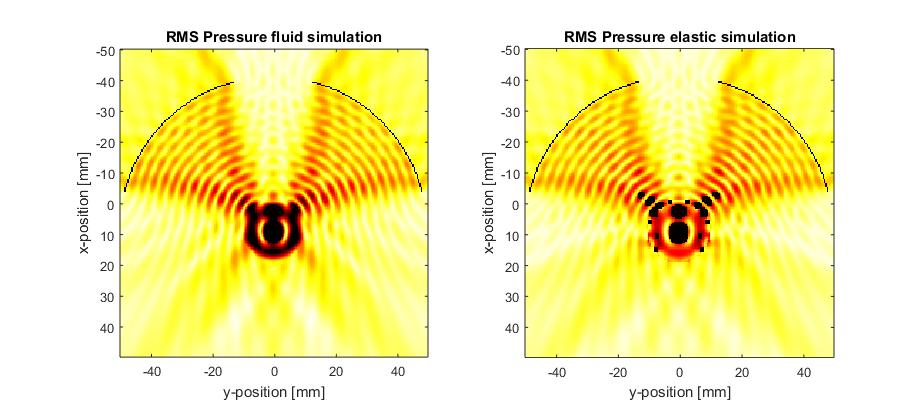
\includegraphics[scale=0.6]{comp_250kHz}
\caption{$f_1  = 0.25$Mhz, $f_2 = 0.25$Mhz.}
\label{comp_250kHz}
\end{figure}
\begin{figure}[H]
\hspace*{-4cm}                                                    
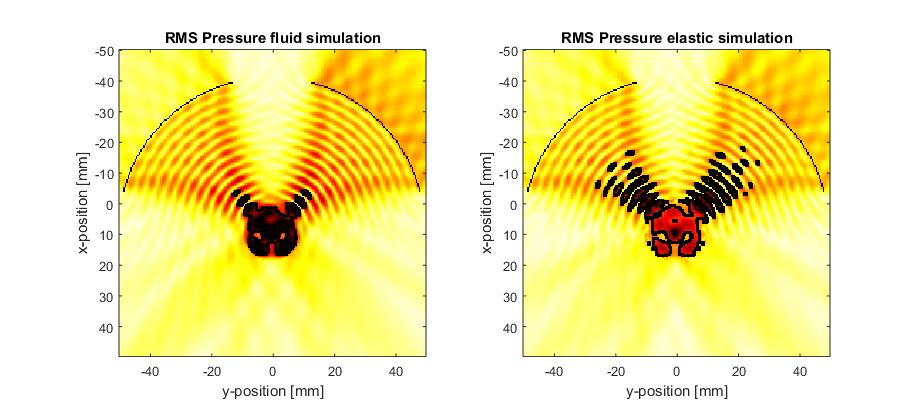
\includegraphics[scale=0.6]{comp_260kHz}
\caption{$f_1  = 0.26$Mhz, $f_2 = 0.25$Mhz.}
\label{comp_260kHz}
\end{figure}
\begin{figure}[H]
\hspace*{-4cm}                                                    
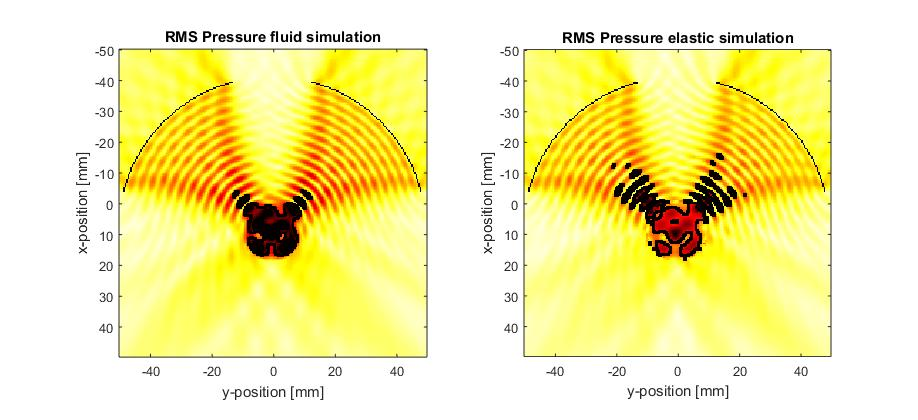
\includegraphics[scale=0.6]{comp_270kHz}
\caption{$f_1  = 0.27$Mhz, $f_2 = 0.25$Mhz.}
\label{comp_270kHz}
\end{figure}
\begin{figure}[H]
\hspace*{-4cm}                                                    
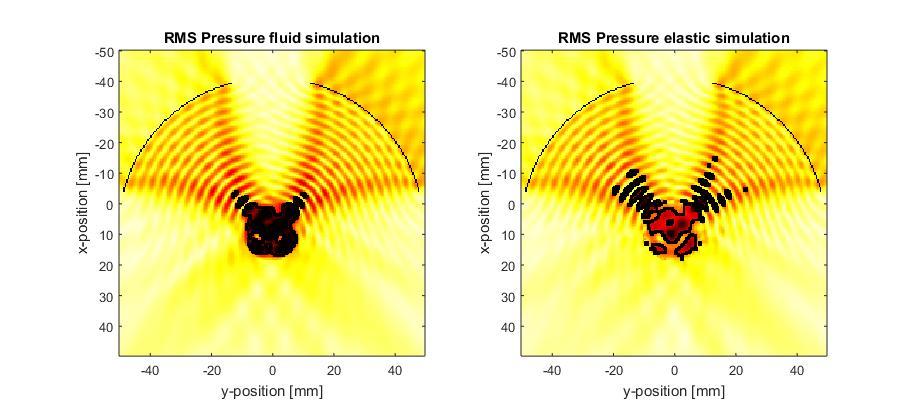
\includegraphics[scale=0.6]{comp_280kHz}
\caption{$f_1  = 0.28$Mhz, $f_2 = 0.25$Mhz.}
\label{comp_280kHz}
\end{figure}
\begin{figure}[H]
\hspace*{-4cm}                                                    
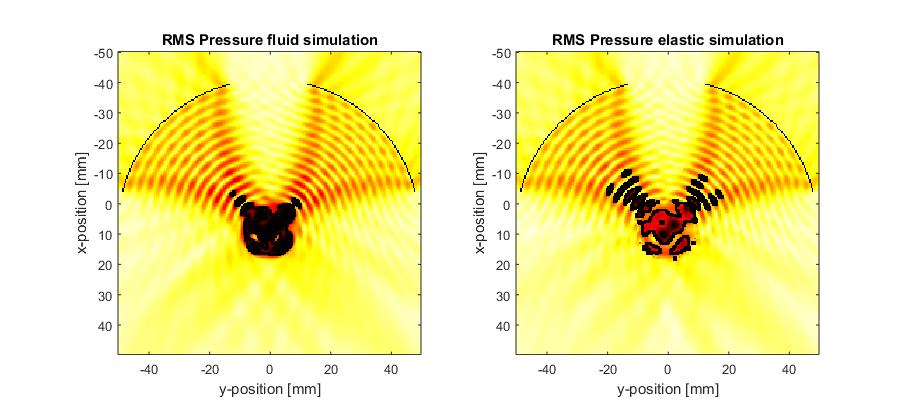
\includegraphics[scale=0.6]{comp_290kHz}
\caption{$f_1  = 0.29$Mhz, $f_2 = 0.25$Mhz.}
\label{comp_290kHz}
\end{figure}
\begin{figure}[H]
\hspace*{-4cm}                                                    
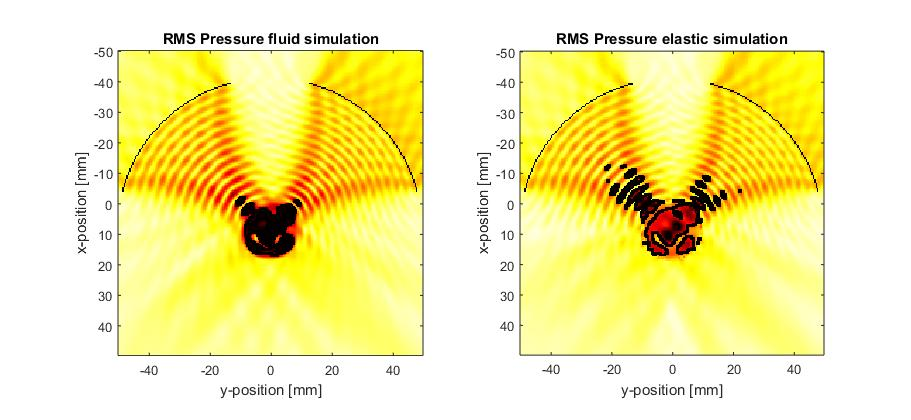
\includegraphics[scale=0.6]{comp_300kHz}
\caption{$f_1  = 0.3$Mhz, $f_2 = 0.25$Mhz.}
\label{comp_300kHz}
\end{figure}


The half-maximum pressure profiles for the inclusion examples were not exactly as expected, with significant side-lobes. This, as I found out by properly reading the user manual, is because the RMS pressure profile is calculated from the entire simulation. In the simulation I've been running, I've started with a non-existent pressure profile, with the US waves then beginning to propagate from the transducers. While this approach is suited to an application that investigated total heat deposition, it gives a bias to the initial waves and is not a good representation of the steady state system. In order to determine the characteristics of the `steady state system', then we need to being the calculations of the time-averaged quantities once the US waves have propagated to the furthest points of the system. 

This can be modified by setting the value sensor.record\_start\_index to the time at which the US field will have reached the furthest point in the computational box. 


\section*{System 3: 2D vertebra shaped inclusion}

The eventual goal of this code is to produce a simulation of ultrasound interacting with a vertebra. We start with 2D simulations to reduce the computational overhead, and plan to progress to three dimensional simulations. In this simulation, we build the environment by importing an image, rather than building the inclusion using one of the in-house functions. I found a simple image of a vertebra online (\href{https://www.cedars-sinai.edu/Patients/Programs-and-Services/Spine-Center/The-Patient-Guide/Anatomy-of-the-Spine/Vertebrae-of-the-Spine.aspx}{Vertebra}), and then modified it to remove colour, mark-ups, and to allow for the placement of the vertebra near the focal point of the two transducers. The image of the vertebra and its placement used for this system is shown in the following \autoref{setup3_image}.

\begin{figure}[H]
\centering
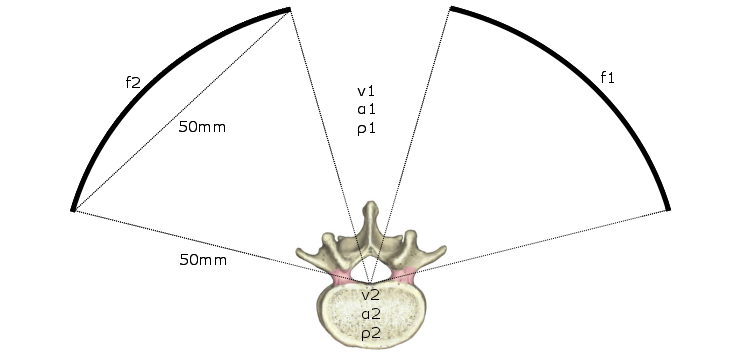
\includegraphics[scale=0.5]{setup3.png}
\caption{I used an online image I found to construct the vertebra, and placed the vertebra approximately at the focus of the transducers.}\label{setup3_image}
\end{figure}

The image of the vertebra was binarized using the matlab function im2bw, where white (zero) represents water and black (one) represents bone, in order to use the image of the vertebra to set the properties of the medium. The im2bw function uses a cut-off to choose whether a point is assigned as 0 (water) or 1. (bone) This cut-off may result in the erroneous assignment of points within the vertebra as 0 or points on the exterior of the vertebra as 1. The image must also be resized such that there is one binary grid point per computational point in the simulation `medium'. As explained in \cite{muir1992modeling,vafaeian2014finite}, the usage of Cartesian grids to represent irregular boundaries can lead to a `staircase' effect, where a boundary that is not aligned with a Cartesian axis becomes irregular. However, these methods use real space calculations whereas the pseudospectral method supposedly only requires two grid points per wavelength, or four points per wavelength for heterogeneous media. I've naively used the binarizing method described above, and performed both fluid and elastic simulations. The RMS pressure results are shown in the following \autoref{fluidvselastic_vertebrae_rms}.

\begin{figure}[H]
\hspace*{-4cm}
\includegraphics[scale=0.7]{fluidvselastic_vertebrae_rms}
\caption{K-wave simulation results using a binary mask of an image of a \href{https://www.cedars-sinai.edu/Patients/Programs-and-Services/Spine-Center/The-Patient-Guide/Anatomy-of-the-Spine/Vertebrae-of-the-Spine.aspx}{vertebra} . The results from the elastic simulation show that the irregular boundary of the vertebra gives erroneous diffraction, absorption, etc. from the inclusion.}\label{fluidvselastic_vertebrae_rms}
\end{figure} 

\autoref{fluidvselastic_vertebrae_rms} displays the result of a simulation in a 512$\times$512 computational grid that is 10cm by 10cm, corresponding to $\Delta x, \Delta y = 0.19$mm. The slowest speed of sound in the simulation is the shear speed of sound in bone, set to $c_s = $ 1500m/s. This means that one wavelength is $\lambda = c_s / f = 1500$ [m/s] / 0.25 $\times 10^6$ Hz = 6mm, and that in this simulation there is a minimum of 31 grid points per wavelength which should be more than sufficient in terms of spatial resolution.  The CFL in this simulation was set to 0.1, below the value suggested in the k-wave user manual (CFL = 0.3 for weakly heterogeneous media). The simulations at this spatial and temporal resolution becomes somewhat computationally costly, with simulations (in Matlab) taking approximately 30 minutes. The results shown in Figure \ref{fluidvselastic_vertebrae_rms} used the smoothing algorithm (Blackman) for the source pressure distribution but not for the medium properties. This is the default setting. I repeated the simulation, adding smoothing for the medium sound speed and the medium density. In the current k-wave configuration, it is not an option to add smoothing from compressional and shear attenuation coefficients. The results from the smoothed vertebra are shown in \autoref{smoothed_vertebrae} (RMS pressure) and in \autoref{max_p_smoothed_vert} (Maximum pressure).

\begin{figure}[H]
\hspace*{-4cm}
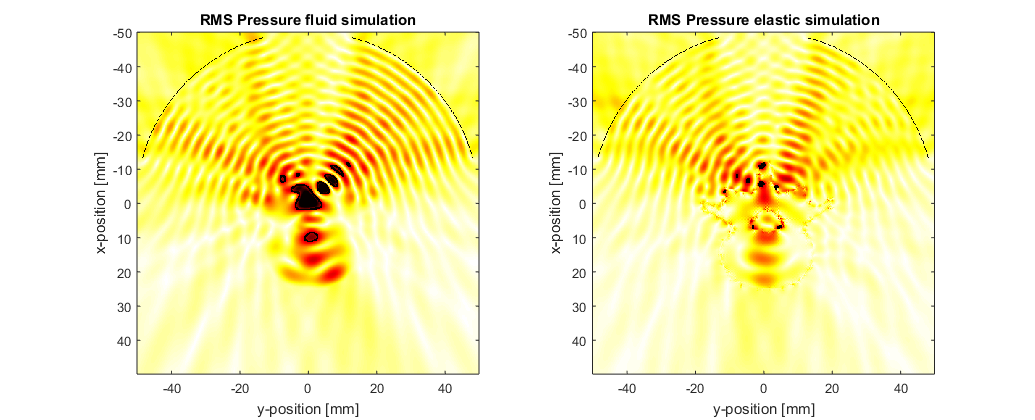
\includegraphics[scale=0.7]{smoothed_vertebrae}
\caption{K-wave simulation RMS pressure results using a binary mask of an image of a \href{https://www.cedars-sinai.edu/Patients/Programs-and-Services/Spine-Center/The-Patient-Guide/Anatomy-of-the-Spine/Vertebrae-of-the-Spine.aspx}{vertebra} . The binary vertebra mask was smoothed in this simulation, but still resulted in strange looking results in the elastic wave propagation simulation.}\label{smoothed_vertebrae}
\end{figure} 

\begin{figure}[H]
\hspace*{-4cm}
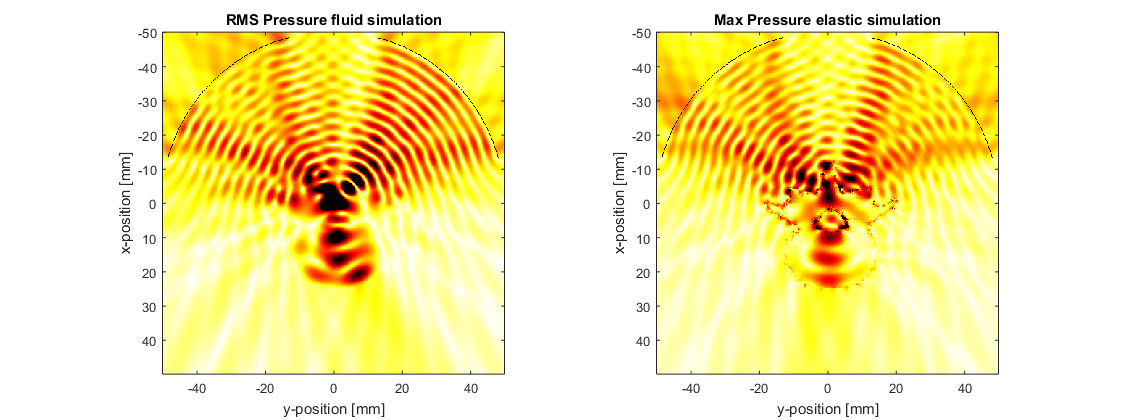
\includegraphics[scale=0.7]{max_p_smoothed_vert}
\caption{K-wave simulation maximum pressure results using a binary mask of an image of a \href{https://www.cedars-sinai.edu/Patients/Programs-and-Services/Spine-Center/The-Patient-Guide/Anatomy-of-the-Spine/Vertebrae-of-the-Spine.aspx}{vertebra} .}\label{max_p_smoothed_vert}
\end{figure} 


In the smoothed medium fluid case the pressure profile is more highly peaked than in the previous un-smoothed case. In both figures (\ref{fluidvselastic_vertebrae_rms} and \ref{smoothed_vertebrae}), the data is normalized to [-1 1], which is why the incoming wave intensity in \ref{smoothed_vertebrae} appears to be lower as it is a smaller fraction of the maximum RMS pressure profile. In the elastic simulation, there are very sharp peaks both inside the vertebra and outside. What is going on here? Is it possible that shear waves are propagating along the interface of the vertebra and constructively interfering at these points? Are these highly peaked maxima the result of standing waves, mode conversion, erroneous assignment of grid points as bone or water? I'd need to perform some tests of the elastic simulation in simpler geometries before I move to real data from the `visible human project' in order to gain a better understanding of shear wave propagation in k-wave. 

\section*{Transducer Optimization}

Since I do not have a pile of time to complete my investigations, I have started to play around with some potential parameters for ultrasound delivery to the spine. There are many parameters that can be optimized, and ideally this procedure would be completed through some sort of machine learning algorithm such as gradient descent with feature normalization, or perhaps some sort of saddle point technique. This approach will become quite complicated, and I won't have time to implement a proper version during this rotation. However, it will still worthwhile to play around with some of the transducer parameters. 

\subsection*{Transducer size}

The first parameter I wanted to investigate is the size of the ultrasound transducer, which I modified by changing the angle each transducer subtended  $\pi/24 \geq \Theta \leq \pi/2$ radians. The two transducers were kept centred at $\pi/4$ radians for transducer 1 and $3\pi/4$ radians for transducer 2. In this case, I kept the frequencies of the two transducers the same $f_1 = f_2 = 0.25$MHz. The metric I am interested in for this trial is the average ultrasound RMS pressure and Maximum pressure within the spinal canal. The results are shown in \autoref{transducer_angle_original}.

\begin{figure}[H]
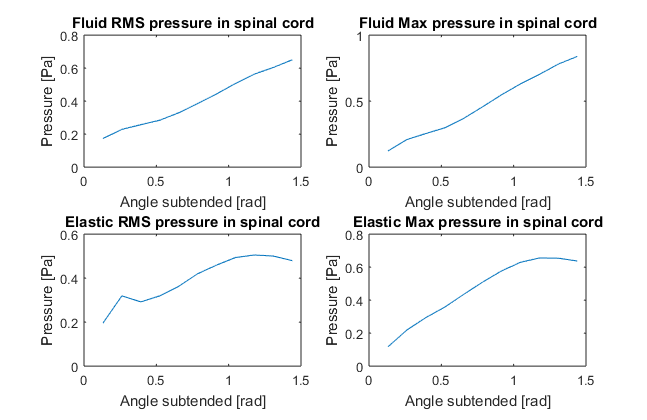
\includegraphics[scale=0.8]{transducer_angle_original}
\caption{The averaged RMS and maximum pressure within the spinal canal for various sizes of transducer, subtending between $\pi/24$ radians and $\pi/2$ radians.}
\end{figure}

In the fluid simulation, the relationship between both RMS pressure and maximum pressure is approximately linear. This is intuitive because by increasing the size of the transducer, we are increasing the total force added to the system. This relationship is slightly difference for the elastic simulation. There is a strange bump at low angles for the RMS pressure that I'm not sure I can explain. Repeating the simulation with higher spatial and temporal resolution might be a good idea. For small angles and maximum pressure, we can see that the relationship between angle subtended and pressure is approximately linear. However, for larger subtended angles we see that the pressure within the spinal canal plateaus and actually drops. This may be due to mode conversion to shear waves along the spinous and transverse processes. Neat. 


Another metric to consider is the RMS and maximum pressure within the spinal canal, normalized by the maximum RMS pressure point and the Maximum pressure point within the entire simulated system. This metric informs the relative efficiency of ultrasound deposition within the spinal canal, and increasing this efficiency is desirable to avoid excess heating of other structures. The results for normalized RMS and maximum pressure within the spinal canal as a function of angle subtended by each transducer is shown in \autoref{transducer_angle_results} for both fluid and elastic simulations.

\begin{figure}[H]
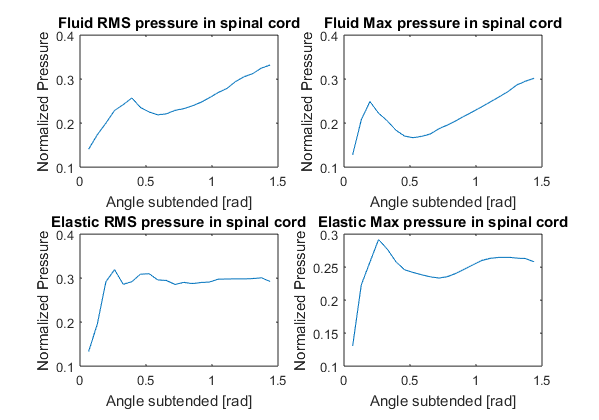
\includegraphics[scale=0.8]{transducer_angle_results}
\caption{The averaged and normalized RMS and maximum pressure within the spinal canal depends on the angle subtended by the transducers. These results are for identical transducers driven at $f_1 = f_2 = 0.25$MHz.} \label{transducer_angle_results}
\end{figure}

Now, these results are from the absolute maxima of the simulation, which is not useful if these maxima occur at the transducer. The transducer pressure was set to 0.5Pa, but it would be worthwhile normalizing by the maximum pressure at the bone-fluid interface because that heating at this interface is the main concern. The results are shown in \autoref{transducer_angle_bonenorm}
\begin{figure}[H]
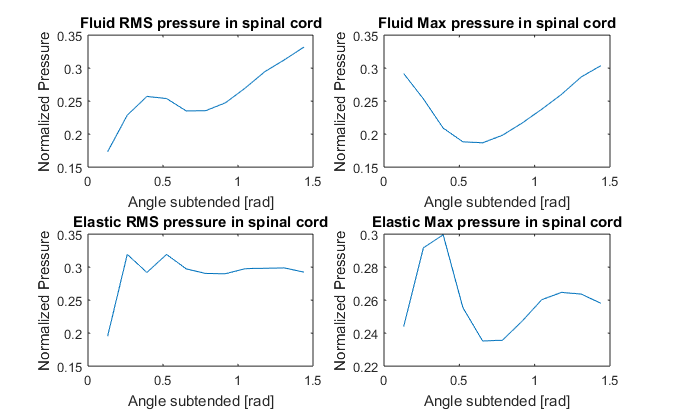
\includegraphics[scale=0.8]{transducer_angle_bonenorm}
\caption{The averaged and normalized (by maximum bone pressure) RMS and maximum pressure within the spinal canal for identical transducers $f_1 = f_2 = $0.25Mhz.} \label{transducer_angle_bonenorm}
\end{figure}
The results when normalized by the maximum intensity along the bone-fluid interface show essentially the same result. The result isn't exactly the same because I used smaller $\Delta \Theta$ steps to speed up the simulation. This suggests that the peak pressure is generally found at the bone-fluid interface. 

\subsection*{Transducer Size and Frequency}

Now, suppose I am interested in optimizing the Transducer size and the frequency $f_1$ as well. I now have a two dimensional parameter space to play with. In this test, I investigate 0.2Mhz$ \geq f_1 \leq $0.3Mhz for the same range of transducer sizes from the previous test. The averaged RMS and maximum pressure within the spinal canal is shown in \autoref{freq_angle_p}
\begin{figure}[H]
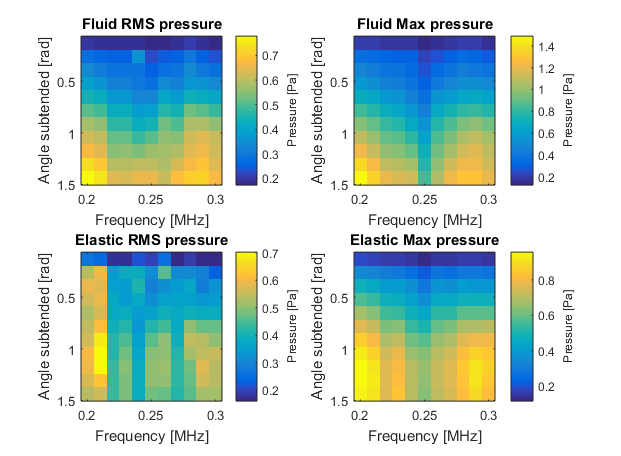
\includegraphics[scale=0.8]{freq_angle_p}
\caption{The average RMS and maximum pressure within the spinal canal for   0.2MHz $\geq f_1 \leq$ 0.3MHz and $f_2 = 0.25$Mhz. The angle subtended by the transducers were increased from $\pi/24$ radians to $\pi/2$ radians}
\label{freq_angle_p}
\end{figure}
\autoref{freq_angle_p} shows a few general trends. The first trend is that the pressure increases as the transducer gets larger. This trend is common among all plots. However, there is a frequency dependence to this relationship. We can see that the slope of this increase is more pronounced for when $f_1 \neq 0.25$Mhz. For example, the pressure maxima in these results generally occur at $f_1 \approx 0.2$Mhz, with local maxima of similar magnitude near $f_1 \approx 0.28$Mhz. Something seems to be going on in the Elastic RMS pressure plot when $f_1 = 0.21$Mhz. The RMS pressures are significantly higher for this frequency than for other frequencies. 

  
In order to glean more information about the safety of the ultrasound propagation, I've normalized the results by the maximum pressure at the bone interface. These normalized results are shown in \autoref{freq_angl_pnorm}. 
\begin{figure}[H]
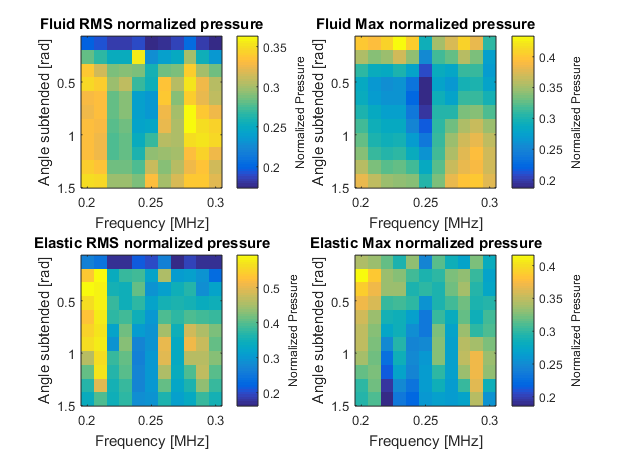
\includegraphics[scale=0.8]{freq_angle_pnorm}
\caption{The averaged  RMS and maximum pressure within the spinal canal for   0.2 MHz $\geq f_1 \leq$ 0.3 MHz and $f_2 = 0.25$ MHz, normalized by the peak pressure at the bone-fluid interface.}
\label{freq_angle_pnorm}
\end{figure}

The normalized results are slightly less clear than the absolute pressure results. This is because normalizing removes the bias towards larger transducers. These results are perhaps better for informing what not to do. For example, excluding the results for the smallest transducer, we see minima around $f_1 = 0.25$ MHz. In the elastic simulation, we again see that when $f_1 = 0.21$ MHz the RMS pressure within the spinal canal is significantly higher than for other frequencies. This is more pronounced in the elastic simulation than the fluid simulation, where we see another peak at 0.28 MHz. The result for $f_1$ = 0.2-0.21 MHz is the only one where the normalized pressure exceeds 50\% of the maximum pressure in the simulation. 

\newpage
\bibliography{lit}{}
\bibliographystyle{ieeetr}





\end{document}